\header{
    \section{Le semeur} \label{le semeur}
    %
    \insertComment{Dans l'esprit anarchiste qui régnait à l'époque, des incidents opposèrent en 1890 les étudiants aux autorités de l'Université, et notamment à Wittmeur, professeur, auteur de la Marche des étudiants.}{Ceux-ci décidèrent d'abandonner ce chant et confièrent à George Garnir, qui devint par la suite rédacteur en chef du "Pourquoi pas ?", le soin de composer un nouvel hymne.}
}

\dualcol{
\enluminure{2}{\href{https://www.youtube.com/watch?v=iw9JGll3oXA}{S}}{emeurs} vaillants du rêve,
\\Du travail, du plaisir,
\\C'est pour nous que se lève
\\La moisson d'avenir;
\\Ami de la science,
\\Léger, insouciant,
\\Et fou d'indépendance
\\Tel est l'étudiant !
\\\\\textbf{Refrain :}
\\Frère, chante ton verre
\\Et chante ta gaîté,
\\La femme qui t'est chère
\\Et la Fraternité
\\A d'autres la sagesse,
\\Nous t'aimons, Vérité,
\\Mais la seule maîtresse,
\\Ah, c'est toi Liberté !
\\\\Aux rêves de notre âge,
\\Larges, ambitieux,
\\S'il était fait outrage
\\Gare à l'audacieux !
\\Si l'on osait prétendre
\\Y mettre le holà,
\\Liberté, pour défendre
\\Tes droits, nous serions là !
\\\\Une aurore nouvelle
\\Grandit à l'horizon;
\\La Science immortelle
\\Eclaire la Raison
\\Rome tremble et chancelle
\\Devant la Vérité;
\\Serrons-nous autour d'elle
\\Contre la papauté !
\bigskip
\bigskip
\bigskip
\begin{center}
\centering
    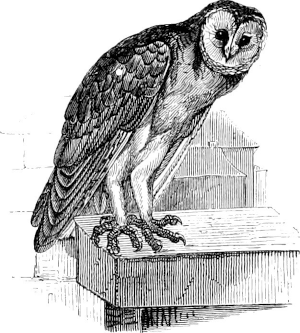
\includegraphics[width=0.3\textwidth]{images/brev60.png}
 \end{center}
}

\breakpage